\documentclass[
	% -- opções da classe memoir --
	12pt,				% tamanho da fonte
	openright,			% capítulos começam em pág ímpar (insere página vazia caso preciso)
	oneside,			% impressão apenas no anverso
	a4paper,			% tamanho do papel.
	% -- opções do pacote babel --
	english,			% idioma adicional para hifenização
	brazil,				% o último idioma é o principal do documento
	]{abntex2}

% ---
% Pacotes fundamentais
% ---
\usepackage{cmap}			% Mapear caracteres especiais no PDF
\usepackage{lmodern}			% Usa a fonte Latin Modern
\usepackage[T1]{fontenc}		% Selecao de codigos de fonte.
\usepackage[utf8]{inputenc}		% Codificacao do documento (conversão automática dos acentos)
\usepackage{lastpage}			% Usado pela Ficha catalográfica
\usepackage{indentfirst}		% Indenta o primeiro parágrafo de cada seção.
\usepackage{color}				% Controle das cores
\usepackage{graphicx}			% Inclusão de gráficos
\usepackage{amsmath}			% Equações
\usepackage{array}				% Colunas de tabela com largura fixa
\usepackage{xurl}				% Quebra de URLs longas nas referências
% ---

% ---
% Pacotes de citações
% ---
\usepackage[brazilian,hyperpageref]{backref}   % Paginas com as citações na bibl
\usepackage[alf]{abntex2cite}	                % Citações padrão ABNT

% ---
% Configurações do pacote backref
% ---
\renewcommand{\backrefpagesname}{Citado na(s) página(s):~}
\renewcommand{\backref}{}
\renewcommand*{\backrefalt}[4]{
	\ifcase #1 %
		Nenhuma citação no texto.%
	\or
		Citado na página #2.%
	\else
		Citado #1 vezes nas páginas #2.%
	\fi}%
% ---

% ---
% Informações de dados para CAPA e FOLHA DE ROSTO
% ---
\titulo{Localizador de Região de Faltas de Alta Impedância \\ como \textit{Firmware} em Microcontrolador Simulado}
\autor{Pedro Henrique Faluba Martins}
\local{Belo Horizonte}
\data{2026}
\instituicao{%
  Universidade Federal de Minas Gerais -- UFMG
  \par
  Escola de Engenharia
  \par
  Curso de Graduação em Engenharia Elétrica}
\tipotrabalho{Relatório Técnico}
\preambulo{}
% ---

% ---
% Configurações de aparência do PDF final
% ---
\definecolor{blue}{RGB}{41,5,195}
\makeatletter
\hypersetup{
		pdftitle={\@title},
		pdfauthor={\@author},
    	pdfsubject={\imprimirpreambulo},
	    pdfcreator={LaTeX with abnTeX2},
		pdfkeywords={abnt}{latex}{abntex}{abntex2}{relatório técnico},
		colorlinks=true,
    	linkcolor=blue,
    	citecolor=blue,
    	filecolor=magenta,
		urlcolor=blue,
		bookmarksdepth=4
}
\makeatother
% ---

% ---
% Espaçamentos entre linhas e parágrafos
% ---
\setlength{\parindent}{1.3cm}
\setlength{\parskip}{0.2cm}

\makeindex

\begin{document}

\frenchspacing

% ----------------------------------------------------------
% ELEMENTOS PRÉ-TEXTUAIS
% ----------------------------------------------------------
\imprimircapa
\imprimirfolhaderosto

\pdfbookmark[0]{\contentsname}{toc}
\tableofcontents*
\cleardoublepage

% ----------------------------------------------------------
% ELEMENTOS TEXTUAIS
% ----------------------------------------------------------
\textual

% ----------------------------------------------------------
% Capítulo 1 - Introdução
% ----------------------------------------------------------
\chapter{Introdução}

As Faltas de Alta Impedância (FAIs) resultam do contato de um condutor energizado com materiais de condutividade muito reduzida e produzem correntes de baixa amplitude, aleatórias e não lineares, o que as torna de difícil detecção e localização pelos sistemas de proteção convencionais \cite{[3]}. Em trabalho anterior \cite{martins_tcc}, propôs-se um procedimento sistemático de seleção de atributos para a localização da região de uma FAI, obtidos exclusivamente a partir das medições da subestação. O resultado foi um conjunto de quinze famílias de atributos, extraídas pelas transformadas discreta de Fourier, de Stockwell e \textit{wavelet} sobre uma janela de 20 ciclos, que superou com folga conjuntos aleatórios de mesma cardinalidade sob validação cruzada aninhada.

Naquele trabalho, argumentou-se ainda que os atributos selecionados não demandam elevado esforço computacional, visto que a extração completa dos 7056 atributos de uma simulação levou em torno de 0,2 s em um processador de uso geral, tempo inferior à própria duração da janela analisada. Esse argumento, porém, foi construído sobre um computador pessoal, enquanto os equipamentos de proteção e monitoramento instalados em subestações são, tipicamente, dispositivos embarcados, baseados em microcontroladores com memória da ordem de centenas de kilobytes e sem sistema operacional. A execução da localização no próprio dispositivo de medição dispensaria a comunicação com um centro de controle e a latência associada a ela, mas não se sabe se as transformadas empregadas, em especial a de Stockwell e a \textit{wavelet}, cabem nos recursos de um dispositivo desse tipo, nem se a seleção de atributos se traduz em economia de recursos em relação ao uso de todos os atributos candidatos.

Além disso, o trabalho anterior entregou um conjunto de atributos, e não um modelo treinado, deixando como trabalho futuro o desenvolvimento de um algoritmo inteligente alimentado por esse conjunto. A escolha desse algoritmo também tem consequências sobre o dispositivo, pois famílias distintas de modelos ocupam memória e demandam processamento em proporções muito diferentes.

Nesse sentido, o objetivo do presente trabalho é implementar o localizador completo, isto é, a extração dos atributos selecionados e um modelo de classificação a jusante, como \textit{firmware} em linguagem C para um microcontrolador ARM Cortex-M4F simulado, e medir a memória e o custo computacional demandados em diferentes configurações. Para isso, verifica-se primeiramente que a implementação embarcada reproduz a implementação de referência em \textit{Python}, e então comparam-se o conjunto selecionado, todos os atributos candidatos, subconjuntos aleatórios e os primeiros atributos do ranqueamento, combinados a quatro famílias de modelos, a diferentes complexidades de modelo e a dois níveis de otimização de compilação.

% ----------------------------------------------------------
% Capítulo 2 - Revisão Bibliográfica
% ----------------------------------------------------------
\chapter{Revisão Bibliográfica}
\label{cap:revisao}
Este capítulo apresenta os conceitos e a literatura necessários para a implementação do localizador em um microcontrolador. Primeiramente, é apresentada a aprendizagem de máquina em microcontroladores e as ferramentas disponíveis para tal. Após, são descritas a arquitetura e as bibliotecas da plataforma adotada, bem como a simulação funcional empregada para executá-la. Por fim, são analisados os trabalhos de localização de FAIs baseados em algoritmos inteligentes quanto ao tratamento dado ao custo computacional.

\section{Aprendizagem de máquina em microcontroladores}
A execução de modelos de aprendizagem de máquina em microcontroladores, denominada \textit{TinyML}, refere-se à inferência em dispositivos com memória da ordem de kilobytes e consumo da ordem de miliwatts, sem sistema operacional e sem comunicação obrigatória com servidores \cite{warden_tinyml}. Segundo \citeonline{ray_tinyml}, a área é motivada justamente pela redução da latência, do consumo de energia e da dependência de conectividade, ao custo de restrições severas de memória e de processamento, que exigem modelos e implementações dedicados.

Dentre as ferramentas disponíveis, destacam-se:

\begin{itemize}
    \item \textbf{TensorFlow Lite Micro:} interpretador de modelos de redes neurais treinados no \textit{TensorFlow}, voltado a microcontroladores e com suporte à quantização em 8 bits, cuja avaliação mostra baixa demanda de recursos e pequeno custo adicional de execução \cite{david_tflm}.

    \item \textbf{CMSIS-NN:} biblioteca de núcleos de redes neurais otimizados para processadores Cortex-M, em ponto fixo de 8 e 16 bits, que reporta ganho de 4,6 vezes em tempo de execução sobre implementações de referência \cite{lai_cmsisnn}.

    \item \textbf{emlearn:} biblioteca que converte modelos treinados no \textit{scikit-learn} \cite{[52]}, como árvores de decisão, florestas aleatórias e redes neurais, em código C sem alocação dinâmica de memória \cite{nordby_emlearn}. Por abranger os modelos clássicos de aprendizagem de máquina, e não apenas redes neurais, é a ferramenta adotada neste trabalho.
\end{itemize}

Quanto à avaliação, o \textit{MLPerf Tiny} estabelece um conjunto padronizado de tarefas e métricas, a saber, acurácia, latência e energia, medidas em dispositivos reais \cite{banbury_mlperf}. Suas tarefas, porém, são de reconhecimento de palavras-chave, detecção visual, classificação de imagens e detecção de anomalias, nas quais a entrada do modelo é o próprio sinal ou um espectrograma simples. Problemas como o deste trabalho, em que a extração dos atributos envolve transformadas tempo-frequência sobre múltiplos canais, não estão representados.

\section{Plataforma Cortex-M4F e CMSIS-DSP}
Os processadores Cortex-M4 implementam a arquitetura Armv7E-M de 32 bits, com \textit{pipeline} de três estágios, instruções dedicadas ao processamento de sinais e unidade de ponto flutuante opcional de precisão simples \cite{arm_cm4}. O microcontrolador STM32F407 integra esse processador, na versão com unidade de ponto flutuante, a 1 MB de memória \textit{flash} e 192 KB de memória RAM, dos quais 64 KB constituem a memória acoplada ao núcleo (CCM), acessível apenas pelo processador e não pelos controladores de acesso direto à memória \cite{st_rm0090}. Trata-se de um microcontrolador de uso difundido e de custo reduzido, o que o torna representativo de um dispositivo de medição embarcado.

Para o processamento de sinais, a biblioteca CMSIS-DSP oferece rotinas otimizadas para a família Cortex-M, dentre as quais a transformada rápida de Fourier (TRF) de sinais reais \cite{arm_cmsisdsp}. Essa transformada, contudo, é disponibilizada apenas para comprimentos que são potências de dois, de 32 a 4096 pontos, restrição relevante para a transformada de Stockwell, conforme discutido no Capítulo \ref{cap:metodologia}.

\section{Simulação funcional de microcontroladores}
O Renode é um simulador que executa o binário compilado para o microcontrolador sem modificações, com modelos dos periféricos de cada plataforma, como as interfaces seriais, e permite automatizar testes por meio do \textit{Robot Framework} \cite{renode}. O simulador contabiliza as instruções executadas pelo processador, mas é funcional e não preciso em ciclos, isto é, reproduz o comportamento do programa sem modelar o \textit{pipeline}, os estados de espera da memória \textit{flash} ou as latências das instruções. Com isso, o número de instruções executadas é adequado à comparação entre configurações, mas não corresponde ao tempo de execução em um dispositivo real.

\section{Custo computacional na localização de FAIs}
A literatura de localização de FAIs baseada em algoritmos inteligentes emprega majoritariamente redes neurais artificiais \cite{[5], [8], [28]}, além de máquinas de vetor de suporte \cite{[27]}, regressão por processos gaussianos \cite{[25]} e comparações entre diferentes algoritmos \cite{[2], [6]}, dentre as quais \citeonline{[6]} opta por um conjunto de árvores de decisão. Esses trabalhos avaliam o desempenho da localização, mas o custo de sua execução é tratado de forma qualitativa. \citeonline{[5]}, por exemplo, destacam a simplicidade e o baixo custo de implementação de seu método, que emprega apenas medições da subestação, sem quantificar a memória ou o processamento exigidos.

Na comparação realizada em \citeonline{martins_tcc}, o processamento exigido pelos trabalhos voltados à região é igualmente descrito em termos das técnicas empregadas e dos pontos de medição necessários, e em nenhum deles foram identificadas medições de memória ou de processamento em um dispositivo embarcado. O próprio trabalho anterior mediu o tempo de extração apenas em um computador pessoal.

\section{Conclusão}
Este capítulo apresentou a aprendizagem de máquina em microcontroladores, a plataforma Cortex-M4F com a biblioteca CMSIS-DSP e a simulação funcional por meio do Renode. Duas observações delimitam a contribuição do presente trabalho. A primeira é que as ferramentas e os \textit{benchmarks} de \textit{TinyML} concentram-se no modelo, enquanto no problema da localização de FAIs a extração dos atributos envolve transformadas tempo-frequência potencialmente mais custosas que o próprio modelo. A segunda é que os trabalhos de localização de FAIs não quantificam a memória e o processamento demandados em um dispositivo embarcado. O presente trabalho mede ambos, sobre o conjunto de atributos obtido em \citeonline{martins_tcc}.

% ----------------------------------------------------------
% Capítulo 3 - Metodologia
% ----------------------------------------------------------
\chapter{Metodologia}
\label{cap:metodologia}
Este capítulo apresenta a metodologia utilizada para implementar o localizador como \textit{firmware} e medir os recursos demandados. Primeiramente são apresentados os dados, os conjuntos de atributos e os modelos avaliados, seguidos da plataforma e da implementação da extração em C. Por fim, são apresentados os procedimentos de verificação da equivalência entre as implementações, o método de medição e a varredura de configurações. A metodologia pode ser, em alto nível, resumida no fluxo apresentado na Figura \ref{fig:pipeline}.

\begin{figure}[htb]
    \centering
    \caption{Fluxo de implementação e avaliação do localizador como \textit{firmware}}
    \label{fig:pipeline}
    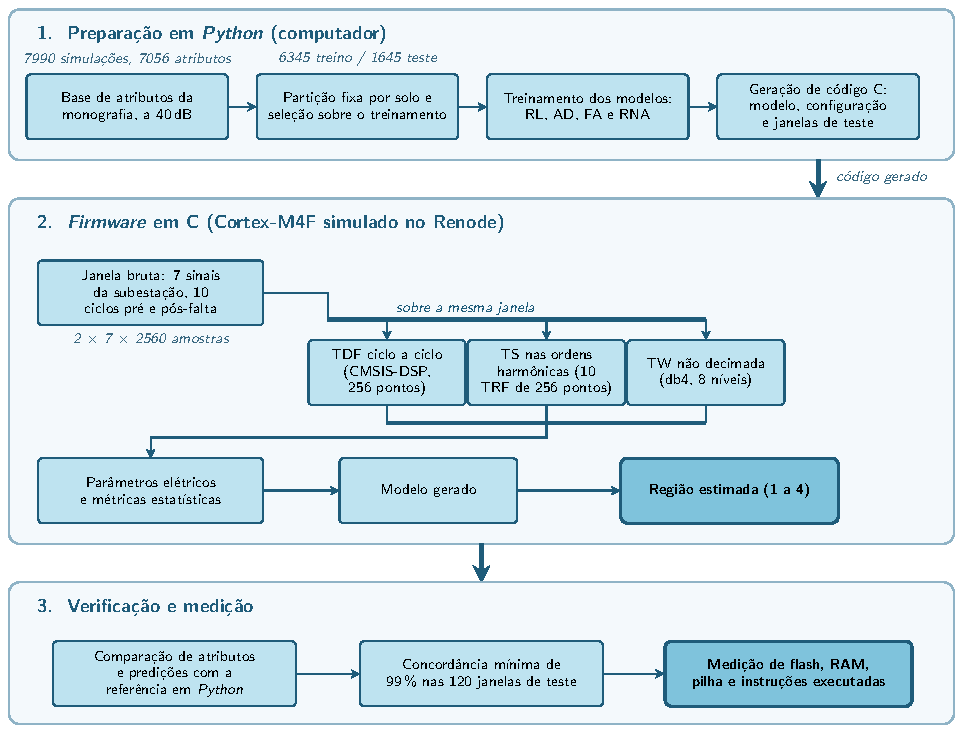
\includegraphics[width=\linewidth]{fig-pipeline.pdf}
    \fonte{Elaborado pelo autor}
\end{figure}

\section{Dados e conjuntos de atributos}
\label{sec:dados}
Foi utilizada a base de atributos construída em \citeonline{martins_tcc}, com 7056 atributos por simulação sobre 7990 simulações de FAIs no sistema teste IEEE de 34 barras adaptado, ao nível de ruído de 40 dB adotado naquele trabalho. A partição entre treinamento e teste foi fixada uma única vez e mantida em todos os experimentos. Ela reserva para o teste sete dos 34 sinais de FAI, sorteados com semente fixa, o que resulta em 6345 simulações de treinamento e 1645 de teste com a mesma proporção de regiões. A partição por sinal de FAI, e não por simulação, impede que uma mesma forma de onda de arco figure simultaneamente no treinamento e no teste.

O ranqueamento publicado em \citeonline{martins_tcc} foi obtido sobre todas as simulações, incluindo, portanto, as que compõem o conjunto de teste deste trabalho. Por essa razão, a cadeia de seleção daquele trabalho, isto é, agrupamento por correlação, filtragem, etapa embutida, etapa \textit{wrapper} e seleção por estabilidade, foi reexecutada sem alterações sobre as simulações de treinamento apenas, ao longo de cem execuções. O índice de estabilidade obtido foi de 0,256, abaixo dos 0,315 obtidos sobre o conjunto completo, o que é esperado diante do menor número de sinais de FAI em cada subamostra, e o conjunto resultante compartilha dez dos quinze agrupamentos com o publicado. Esse conjunto, apresentado na Tabela \ref{tab:top15}, é o conjunto de referência deste trabalho.

\begin{table}[htb]
\IBGEtab{%
  \caption{Conjunto de quinze atributos selecionado sobre as simulações de treinamento}%
  \label{tab:top15}%
}{%
  \begin{tabular}{cllllll}
  \toprule
  \textbf{\#} & \textbf{$\pi$} & \textbf{Técnica} & \textbf{Parâmetro} & \textbf{Canal} & \textbf{Ordem} & \textbf{Métrica} \\
  \midrule \midrule
  1 & 0,95 & TDF & Módulo da impedância & $V_f$ / $I_f$ & h1 & máximo \\
  2 & 0,76 & TW & Módulo & $V_f$ & D3 & diferença \\
  3 & 0,68 & TS & DHT & $I_f$ & todas & razão \\
  4 & 0,48 & TW & Módulo & $I_n$ & D7 & máximo \\
  5 & 0,43 & TW & Módulo da impedância & $V_f$ / $I_f$ & D6 & razão \\
  6 & 0,38 & TW & Energia & $I_f$ & D8 & amplitude \\
  7 & 0,35 & TDF & Módulo da impedância & $\Sigma V$ / $I_n$ & h3 & média \\
  8 & 0,29 & TS & Módulo da impedância & $\Sigma V$ / $I_n$ & h3 & razão \\
  9 & 0,25 & TDF & Energia & $V_f$ & h1 & máximo \\
  10 & 0,21 & TS & Energia & $V_f$ & h8 & média \\
  11 & 0,21 & TS & Módulo & $V_2$ & h12 & diferença \\
  12 & 0,20 & TS & Ângulo & $I_n$ & h1 & média \\
  13 & 0,19 & TDF & Ângulo & $V_f$ & h1 & média \\
  14 & 0,19 & TS & Módulo & $V_2$ & h10 & diferença \\
  15 & 0,15 & TDF & Energia & $V_2$ & h14 & média \\
  \bottomrule
  \end{tabular}%
}{\fonte{Elaborado pelo autor. $\pi$: frequência de seleção nas cem execuções; TDF, TS e TW: transformadas discreta de Fourier, de Stockwell e \textit{wavelet}; $V_f$ e $I_f$: tensão e corrente da fase faltosa; $I_n$: corrente de neutro; $\Sigma V$: soma das tensões trifásicas; $V_2$: tensão de sequência negativa; h$n$: ordem harmônica; D$n$: banda diádica da TW.}}
\end{table}

Além do conjunto de referência, foram avaliados o conjunto publicado em \citeonline{martins_tcc}, mantido apenas como comparação por ter sido selecionado com acesso às simulações de teste, todos os 7056 atributos candidatos, os primeiros três, cinco e dez atributos do conjunto de referência e dez subconjuntos de quinze atributos sorteados uniformemente dentre os 7056, cada um com semente fixa.

\section{Modelos de classificação}
Foram avaliadas quatro famílias de modelos, todas treinadas com o \textit{scikit-learn} \cite{[52]} e com ponderação das classes:

\begin{itemize}
    \item \textbf{Regressão logística (RL):} com regularização L2, por ser o classificador de referência empregado na etapa \textit{wrapper} de \citeonline{martins_tcc}.

    \item \textbf{Árvore de decisão (AD):} com profundidade máxima de oito níveis.

    \item \textbf{Floresta aleatória (FA):} com trinta árvores de profundidade máxima oito, cuja predição é a média das proporções de classe das folhas.

    \item \textbf{Rede neural artificial (RNA):} perceptron com uma camada oculta de dezesseis neurônios e ativação ReLU.
\end{itemize}

A RL e a RNA recebem os atributos após a transformação logarítmica com sinal e a padronização adotadas em \citeonline{martins_tcc}. Já a AD e a FA recebem os atributos sem transformação, visto que árvores de decisão são invariantes a transformações monotônicas, o que dispensa quinze cálculos de logaritmo por janela no dispositivo.

A conversão para C empregou o emlearn \cite{nordby_emlearn} para a AD e a FA. Para a RL, não suportada pela biblioteca, e para a RNA, foram gerados os coeficientes e uma rotina própria de inferência. No caso da RNA, a rotina do emlearn exige que os vetores intermediários tenham a largura da camada de entrada, o que, com os 7056 atributos, demandaria 55 KB adicionais de RAM.

\section{Plataforma e implementação da extração}
\label{sec:implementacao}
O \textit{firmware} foi desenvolvido para o STM32F407, simulado no Renode a partir da plataforma da placa de desenvolvimento STM32F4 Discovery, e compilado com otimização para tamanho, unidade de ponto flutuante de precisão simples por \textit{hardware} e eliminação de código não utilizado. Todas as variáveis são estáticas, sem alocação dinâmica de memória. O modelo de plataforma do simulador dispõe de mais memória que o microcontrolador real e não contém a memória CCM. Por isso, a CCM foi acrescentada ao modelo, e os limites reais de 1 MB de \textit{flash} e 128 KB de RAM principal foram impostos na ligação do programa.

A extração em C é genérica, isto é, capaz de calcular qualquer um dos 7056 atributos. O conjunto a ser calculado é descrito por uma tabela gerada automaticamente a partir dos atributos do modelo, que indica, para cada transformada, os canais e as ordens harmônicas ou bandas necessárias. Somente essas combinações são calculadas, e os vetores de trabalho são dimensionados por elas. As três transformadas foram implementadas como segue:

\begin{itemize}
    \item \textbf{TDF:} aplicada ciclo a ciclo por meio da TRF de sinais reais da CMSIS-DSP, com 256 pontos.

    \item \textbf{TS:} em \citeonline{martins_tcc}, cada voz harmônica é obtida por uma transformada inversa de 2560 pontos, comprimento de dez ciclos que não é potência de dois. A transformada direta de 2560 pontos foi obtida por decimação, a partir de dez TRFs de 256 pontos. Como apenas a média de cada voz em cada ciclo é utilizada, a transformada inversa foi substituída por uma forma fechada, dada pela Equação \eqref{eq:ts}, em que $H$ é a transformada direta, $k_0 = 10h$ é a raia do harmônico $h$, $G_h$ é a janela gaussiana da transformada \cite{[54]}, $B$ é a média de um termo exponencial sobre as 256 amostras de um ciclo e $c$ é o ciclo. A soma foi truncada em $|m| \leq 1{,}5\,k_0$, onde a janela gaussiana vale $e^{-44}$, contribuição desprezível em precisão simples.
    \begin{equation}
        X_{h,c} = \frac{2}{N} \sum_{|m| \leq 15h} H[k_0 + m]\, G_h[m]\, B[m]\, e^{j 2\pi m c / 10}
        \label{eq:ts}
    \end{equation}

    \item \textbf{TW:} implementada na forma não decimada, por convolução circular com os filtros da Daubechies de quarta ordem sobreamostrados a cada nível, com o valor eficaz de cada ciclo acumulado durante a própria filtragem, sem armazenar as bandas.
\end{itemize}

As componentes de sequência negativa da TW, que demandam a rotação de fase pela transformada de Hilbert, empregam a transformada inversa de 2560 pontos obtida pela mesma decimação. Todos os cálculos são realizados em precisão simples.

\section{Verificação da equivalência}
\label{sec:verificacao}
A implementação de referência foi reescrita em \textit{Python}, sem dependência do código de \citeonline{martins_tcc}, e reproduz a matriz de atributos daquele trabalho, em todas as 1645 simulações de teste e todos os 7056 atributos, com erro relativo máximo de $6{,}9 \times 10^{-8}$, correspondente ao arredondamento do armazenamento em precisão simples. Cada rotina em C possui uma contraparte nessa referência, e os algoritmos reformulados, isto é, a decimação e a forma fechada da TS, foram verificados contra as definições com erro da ordem do arredondamento em precisão dupla.

A referência é calculada sobre a mesma janela em precisão simples recebida pelo dispositivo, de modo que apenas a aritmética da implementação em C difere entre as duas. Um atributo calculado em C, $c$, é considerado equivalente ao de referência, $p$, quando $|c - p| \leq 10^{-3}|p| + 10^{-3}\sigma$, em que $\sigma$ é o desvio padrão do atributo no conjunto de teste, sendo os ângulos comparados por diferença envolvente. O termo proporcional a $\sigma$ é necessário porque atributos de diferença, de curtose e angulares assumem valores próximos de zero, nos quais o erro relativo isolado é instável.

Cada janela bruta ocupa 140 KB, de modo que apenas seis ou sete janelas cabem na \textit{flash} ao lado do programa. Foram selecionadas 120 janelas do conjunto de teste, estratificadas por região, executadas em lotes, cada qual compilado em um \textit{firmware} distinto. Uma configuração foi considerada válida quando a predição do dispositivo concorda com a do \textit{scikit-learn} em ao menos 99\% dessas janelas.

\section{Método de medição}
\label{sec:medicao}
As métricas adotadas, bem como a forma de obtenção de cada uma, foram:

\begin{itemize}
    \item \textbf{Memória \textit{flash}:} soma das seções de código e de dados constantes, obtida a partir do mapa de ligação e separada por módulo, isto é, extração, CMSIS-DSP, modelo, biblioteca padrão e aplicação, excluídas as janelas de teste.

    \item \textbf{RAM estática:} soma das variáveis inicializadas e não inicializadas, incluindo a CCM, obtida da mesma forma.

    \item \textbf{Pilha:} pico de utilização, medido pelo preenchimento prévio da região da pilha com um padrão conhecido e pela verificação, ao final da execução, da porção sobrescrita.

    \item \textbf{Instruções executadas:} lidas do contador do simulador por uma rotina associada ao endereço de uma função de marcação, executada no instante exato em que o processador a alcança. A extração foi medida como a média sobre as janelas do lote, executadas duas vezes, e a inferência como a média sobre os atributos de referência de até 1645 simulações de teste, visto que o custo de uma árvore depende do caminho percorrido. Uma janela adicional foi medida com marcações entre as etapas da extração.
\end{itemize}

A precisão da leitura do contador foi verificada sobre um laço de comprimento conhecido. A alternativa de pausar a simulação ao surgir uma mensagem na interface serial mostrou-se imprecisa, pois o simulador interrompe a execução apenas em seu próximo ponto de sincronização, até milhões de instruções depois.

Vale ressaltar que o número de instruções não equivale ao tempo de execução em um dispositivo real. Em um STM32F407 a 168 MHz, o tempo depende ainda do esvaziamento do \textit{pipeline} a cada desvio, dos estados de espera da \textit{flash}, apenas parcialmente ocultados pelo seu acelerador, e das latências das instruções, que vão de um ciclo para operações inteiras simples a quatorze ciclos para a divisão e a raiz quadrada em ponto flutuante. Por isso, as estimativas de tempo apresentadas assumem uma instrução por ciclo e são tratadas apenas como estimativas grosseiras.

\section{Varredura de configurações}
A varredura avaliou 80 configurações, organizadas em três grupos, cada um variando um fator por vez:

\begin{itemize}
    \item \textbf{Conjunto de atributos e modelo:} os dezesseis conjuntos da Seção \ref{sec:dados}, combinados às quatro famílias de modelos, com otimização para tamanho, totalizando 64 configurações.

    \item \textbf{Complexidade do modelo:} sobre o conjunto de referência, FA com 5, 10 e 30 árvores e profundidades de 4, 8 e 12, AD com profundidades de 4 e 12 e RNA com 8 e 32 neurônios.

    \item \textbf{Otimização de compilação:} as quatro famílias de modelos sobre o conjunto de referência, compiladas com otimização para velocidade.
\end{itemize}

Cada configuração é treinada, convertida, executada no dispositivo simulado sobre as 120 janelas e medida de forma automatizada. O comprimento da janela não foi variado, visto que a amostragem de 256 amostras por ciclo e a janela de 20 ciclos integram a própria definição dos atributos de \citeonline{martins_tcc}.

\section{Conclusões}
Este capítulo apresentou a metodologia empregada para implementar e avaliar o localizador como \textit{firmware}. O conjunto de referência foi obtido pela mesma cadeia de seleção de \citeonline{martins_tcc}, executada apenas sobre as simulações de treinamento, e foi combinado a quatro famílias de modelos. A extração foi implementada em C sobre a CMSIS-DSP, com as transformadas reformuladas para comprimentos e operações compatíveis com o microcontrolador, e a equivalência com a referência em \textit{Python} é verificada em cada configuração antes de qualquer medição. O capítulo seguinte apresenta os resultados obtidos.

% ----------------------------------------------------------
% Capítulo 4 - Resultados e Discussão
% ----------------------------------------------------------
\chapter{Resultados e Discussão}
Este capítulo apresenta os resultados obtidos de cada etapa da metodologia, iniciando pela equivalência entre as implementações, seguida do custo da configuração de referência e dos efeitos do conjunto de atributos, da complexidade do modelo e da otimização de compilação.

\section{Equivalência entre as implementações}
As quatro famílias de modelos, convertidas para C e alimentadas pelo conjunto de referência, concordaram com o \textit{scikit-learn} em todas as 1645 simulações de teste, tanto compiladas para o computador quanto executadas no dispositivo simulado. Ao longo da varredura, apenas oito das 25 configurações com FA divergiram, em uma a quatro das 1645 simulações, sempre de forma idêntica no computador e no dispositivo. A divergência decorre da representação em 8 bits das proporções de classe das folhas pelo emlearn, que inverte a decisão quando duas regiões estão praticamente empatadas, e não de um erro da implementação.

Os quinze atributos do conjunto de referência calculados no dispositivo atenderam ao critério de equivalência em todos os 1800 valores das 120 janelas, com o maior desvio correspondendo a 11,5\% da tolerância. Esse desvio ocorre no módulo da impedância entre a soma das tensões e a corrente de neutro, já que a soma das três tensões de fase, de aproximadamente 21 kV, cancela-se em um resíduo pequeno, cuja resolução em precisão simples é limitada.

Estendida aos 7056 atributos, a verificação atendeu ao critério em 99,99\% dos valores. Os 244 atributos que falharam em ao menos uma janela concentram-se em impedâncias entre grandezas que se cancelam, como a soma das tensões e as componentes de sequência negativa, e em momentos estatísticos de séries quase constantes. Nesses atributos, o erro da aritmética em precisão simples é, em mediana, cerca de sete vezes maior que o produzido apenas pelo armazenamento da janela em precisão simples, o que constitui um limite da representação numérica, e não da implementação. Ainda assim, todas as 80 configurações da varredura atenderam ao critério de concordância das predições, com mínimo de 99,17\%, correspondente a uma divergência em 120 janelas, ocorrida em uma das FAs mencionadas acima.

\section{Custo da configuração de referência}
A Tabela \ref{tab:referencia} apresenta os recursos demandados pelo conjunto de referência com cada família de modelos.

\begin{table}[htb]
\IBGEtab{%
  \caption{Recursos demandados pelo conjunto de referência}%
  \label{tab:referencia}%
}{%
  \begin{tabular}{lcccc}
  \toprule
  & \textbf{RL} & \textbf{AD} & \textbf{FA} & \textbf{RNA} \\
  \midrule \midrule
  macro-F1 & 0,680 & 0,741 & 0,781 & 0,689 \\
  \midrule
  \textit{Flash} total (KB) & 18,8 & 21,9 & 131,5 & 19,9 \\
  \midrule
  \textit{Flash} do modelo (KB) & 0,6 & 3,7 & 113,2 & 1,7 \\
  \midrule
  RAM estática (KB) & 97,3 & 97,3 & 97,3 & 97,5 \\
  \midrule
  Pico de pilha (B) & 1800 & 1800 & 1800 & 1800 \\
  \midrule
  Instruções por extração (milhões) & 17,17 & 17,17 & 17,17 & 17,17 \\
  \midrule
  Instruções por inferência & 1648 & 219 & 2717 & 3828 \\
  \bottomrule
  \end{tabular}%
}{\fonte{Elaborado pelo autor. macro-F1 sobre as 1645 simulações de teste.}}
\end{table}

A extração dos atributos demanda 17,17 milhões de instruções por janela, enquanto a inferência demanda de 219 a 3828 instruções, isto é, cerca de 0,02\% do total no pior caso. O custo do localizador é, portanto, determinado pela extração, e não pelo modelo. Mesmo na RL, o modelo mais simples em memória, a maior parte das instruções de inferência corresponde aos quinze cálculos de logaritmo da transformação de entrada, e não à combinação linear em si. A Figura \ref{fig:custo} detalha essa distribuição por etapa da extração.

\begin{figure}[htb]
    \centering
    \caption{Instruções executadas por janela, por etapa da extração e na inferência}
    \label{fig:custo}
    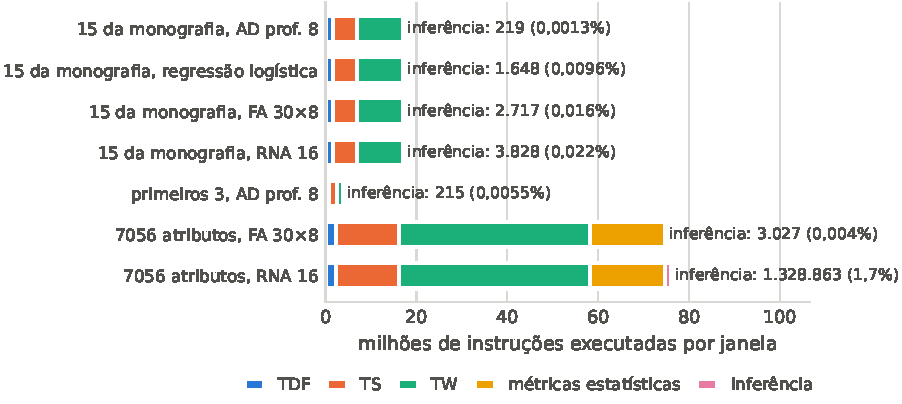
\includegraphics[width=0.95\linewidth]{fig-custo-etapas.pdf}
    \fonte{Elaborado pelo autor}
\end{figure}

No conjunto de referência, a TW responde por 60\% das instruções da extração, a TS por 31\%, a TDF por 9\% e as métricas estatísticas por apenas 0,2\%. O peso da TW decorre da forma não decimada, em que cada um dos até oito níveis filtra todas as 2560 amostras de cada janela. A TS, cuja definição exige uma transformada inversa por harmônico, responde por menos de um terço do total por meio da forma fechada da Equação \eqref{eq:ts}, mesmo sendo a DHT calculada sobre as vinte ordens harmônicas. Vale ressaltar que a própria implementação influencia esses números, já que a remoção do tratamento circular de índices no interior da filtragem da TW reduziu as instruções dessa etapa em 32\%, com resultados idênticos.

Quanto à memória, a \textit{flash} do conjunto de referência é dominada pelo modelo no caso da FA, de 113,2 KB, enquanto a extração ocupa 4,0 KB, a CMSIS-DSP 5,8 KB e a biblioteca padrão 7,3 KB. Já a RAM estática, de aproximadamente 97 KB em todas as famílias, corresponde quase integralmente aos vetores de trabalho da extração, isto é, os coeficientes das transformadas de cada canal, as tabelas gaussianas da TS e os vetores intermediários da TW. Em uma estimativa grosseira, à razão de uma instrução por ciclo a 168 MHz, a extração levaria cerca de 102 ms, abaixo dos aproximadamente 333 ms de sinal contidos nas duas janelas.

\section{Efeito do conjunto de atributos}
A Tabela \ref{tab:conjuntos} apresenta o desempenho de cada conjunto de atributos com cada família de modelos, juntamente com as instruções de extração, e a Figura \ref{fig:f1-instrucoes} relaciona o desempenho ao custo computacional de todas as configurações.

\begin{table}[htb]
\IBGEtab{%
  \caption{Desempenho e custo de extração por conjunto de atributos}%
  \label{tab:conjuntos}%
}{%
  \begin{tabular}{lccccc}
  \toprule
  \textbf{Conjunto} & \textbf{RL} & \textbf{AD} & \textbf{FA} & \textbf{RNA} & \textbf{Instruções (milhões)} \\
  \midrule \midrule
  Referência (15) & 0,680 & 0,741 & 0,781 & 0,689 & 17,2 \\
  \midrule
  Publicado (15) & 0,694 & 0,706 & 0,755 & 0,737 & 16,4 \\
  \midrule
  Primeiros 10 & 0,639 & 0,699 & 0,776 & 0,669 & 16,0 \\
  \midrule
  Primeiros 5 & 0,577 & 0,687 & 0,706 & 0,594 & 11,8 \\
  \midrule
  Primeiros 3 & 0,467 & 0,572 & 0,577 & 0,488 & 3,9 \\
  \midrule
  Aleatórios (15), média & 0,389 & 0,423 & 0,452 & 0,402 & 18,9 \\
  \midrule
  Aleatórios (15), máximo & 0,429 & 0,484 & 0,491 & 0,445 & 33,8 \\
  \midrule
  Todos (7056) & 0,653 & 0,780 & 0,754 & 0,632 & 74,8 \\
  \bottomrule
  \end{tabular}%
}{\fonte{Elaborado pelo autor. Valores de macro-F1 sobre as 1645 simulações de teste. Instruções de extração por janela; para os conjuntos aleatórios, mediana e máximo dos dez sorteios.}}
\end{table}

\begin{figure}[htb]
    \centering
    \caption{Desempenho em função das instruções executadas por janela}
    \label{fig:f1-instrucoes}
    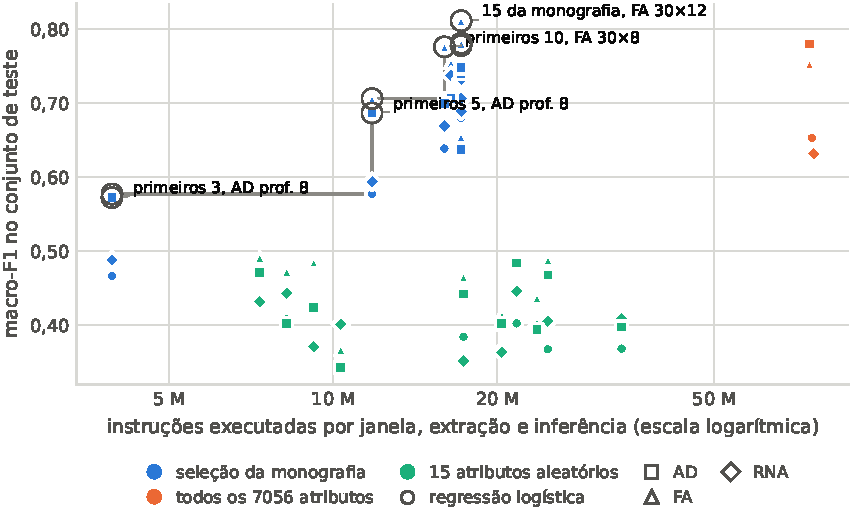
\includegraphics[width=0.95\linewidth]{fig-f1-instrucoes.pdf}
    \fonte{Elaborado pelo autor. Os pontos circundados formam a fronteira de configurações não superadas simultaneamente em desempenho e custo.}
\end{figure}

O conjunto de referência superou todos os dez conjuntos aleatórios em todas as famílias de modelos, visto que mesmo o seu pior resultado, de 0,680 com a RL, supera o melhor resultado aleatório, de 0,491 com a FA. Esse resultado é ainda mais relevante quando se observa que os conjuntos aleatórios demandam entre 7,3 e 33,8 milhões de instruções, com mediana de 18,9 milhões, isto é, custo comparável ao do conjunto de referência. A seleção, portanto, não reduz o custo em relação a um conjunto arbitrário de mesma cardinalidade, mas concentra nele a informação sobre a região.

Em relação aos 7056 atributos candidatos, o conjunto de referência demanda 4,4 vezes menos instruções e não perde desempenho. A FA alcança 0,781 com o conjunto de referência e 0,754 com todos os atributos, enquanto a AD alcança 0,741 e 0,780, respectivamente, a única família em que o conjunto completo é superior. Além disso, o conjunto completo exige de 139 a 167 KB de RAM estática, que só cabem no microcontrolador com o uso da CCM, e de 63 a 557 KB de \textit{flash}, conforme o modelo. Na extração dos 7056 atributos, as métricas estatísticas passam a responder por 22\% das instruções, contra 0,2\% no conjunto de referência.

Os primeiros atributos do ranqueamento mostram que o custo pode ser reduzido com perda gradual de desempenho. Os dez primeiros alcançam 0,776 com a FA, praticamente o mesmo resultado do conjunto completo de quinze, com 16,0 milhões de instruções, enquanto os cinco primeiros alcançam 0,706 com 11,8 milhões e os três primeiros, 0,577 com 3,9 milhões. A redução é mais acentuada nos três primeiros porque estes dispensam a maior parte das bandas da TW e das vozes da TS. Já o conjunto publicado obteve desempenho próximo ao de referência, superior com a RL e a RNA e inferior com a AD e a FA, sendo que essa comparação é otimista para o conjunto publicado, selecionado com acesso às simulações de teste.

A Figura \ref{fig:f1-flash} relaciona o mesmo desempenho à memória \textit{flash}. Diferentemente das instruções, a \textit{flash} pouco varia com o conjunto de atributos, situando-se entre 18 e 22 KB para todos os conjuntos de quinze atributos, exceto com a FA. Isso ocorre porque o código de extração é o mesmo para qualquer conjunto, variando apenas a tabela que o configura. Com isso, a \textit{flash} é determinada pelo modelo, enquanto a seleção de atributos determina as instruções executadas e a RAM.

\begin{figure}[htb]
    \centering
    \caption{Desempenho em função da memória \textit{flash} ocupada}
    \label{fig:f1-flash}
    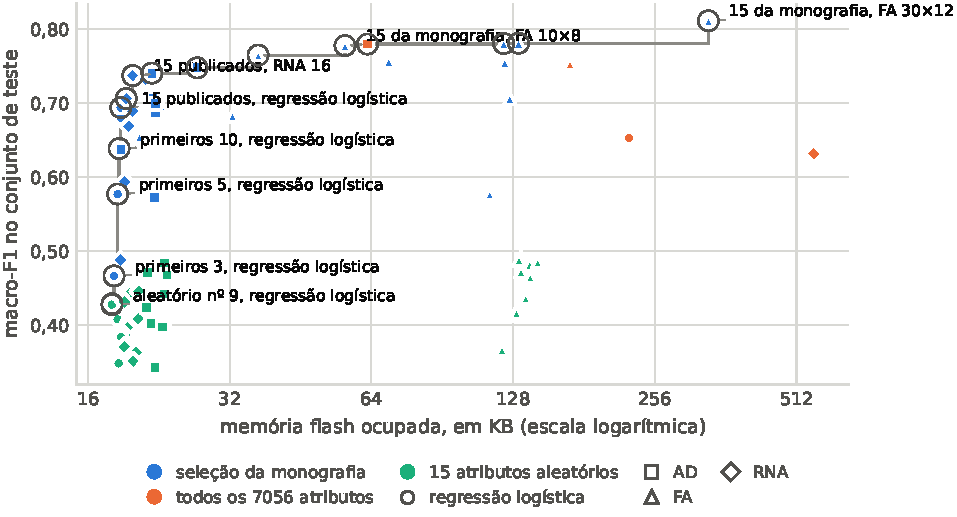
\includegraphics[width=0.95\linewidth]{fig-f1-flash.pdf}
    \fonte{Elaborado pelo autor}
\end{figure}

\section{Complexidade do modelo e otimização de compilação}
Na FA, o aumento de 5 para 30 árvores e de profundidade 4 para 12 elevou o macro-F1 de 0,655 para 0,812, o melhor resultado da varredura, ao custo de 314 KB de \textit{flash} para o modelo, contra 2,4 KB da menor configuração. Os ganhos, contudo, não são uniformes. Com dez árvores de profundidade oito, a FA alcança 0,778 com 38 KB, enquanto as trinta árvores de mesma profundidade acrescentam apenas 0,003 ao custo de 75 KB adicionais. Na AD, a profundidade 4 resultou em 0,637 e a profundidade 12 em 0,748, próxima dos 0,741 da profundidade 8. Na RNA, oito, dezesseis e trinta e dois neurônios resultaram em 0,706, 0,689 e 0,733, sem tendência monotônica. Em todos os casos, a inferência permaneceu abaixo de 6300 instruções, de modo que a complexidade do modelo afeta essencialmente a \textit{flash}.

A otimização para velocidade elevou as instruções de extração em 3,2\%, de 17,17 para 17,71 milhões, reduziu as instruções de inferência da AD em 31\% e acrescentou de 1,3 a 9,3 KB de \textit{flash}. O aumento das instruções de extração não significa que o código seja mais lento, já que esse nível de otimização reorganiza o código para reduzir ciclos por meio de desvios e acessos à memória, efeito que o simulador funcional não captura. Esse resultado ilustra a limitação discutida na Seção \ref{sec:medicao}.

\section{Adequação a dispositivos embarcados}
O \textit{firmware} de todas as 80 configurações coube no STM32F407, com no máximo 557 KB de \textit{flash} e 169 KB de RAM estática somada à pilha, sendo a CCM necessária apenas com os 7056 atributos. Nenhuma configuração caberia, contudo, em um microcontrolador de 32 KB de RAM, típico da classe Cortex-M0+, visto que a menor RAM estática observada foi de 49 KB.

Há, porém, um requisito que não está contabilizado nesses valores. Neste trabalho, as janelas brutas residem na \textit{flash} como dados de teste, mas um dispositivo real precisaria mantê-las em RAM, à medida que fossem adquiridas. As duas janelas dos sete sinais ocupam de 120 a 140 KB em precisão simples, conforme os canais exigidos pelo conjunto, valor que, somado aos vetores de trabalho da extração, excede a RAM do microcontrolador adotado.

\section{Conclusões}
Este capítulo apresentou os resultados obtidos. A implementação em C reproduziu a referência em \textit{Python} em todas as configurações avaliadas, com a única ressalva de atributos cujo cálculo é sensível à precisão simples. O custo do localizador é determinado pela extração dos atributos, que demanda cerca de 17 milhões de instruções por janela no conjunto de referência, contra no máximo alguns milhares na inferência. O conjunto de referência superou todos os conjuntos aleatórios de mesma cardinalidade, a custo comparável, e superou o conjunto completo de atributos em três das quatro famílias, a menos de um quarto do custo. Por fim, a \textit{flash} é determinada pelo modelo e a RAM pela extração, e o armazenamento da janela bruta constitui o principal obstáculo a uma implementação em um dispositivo real.

% ----------------------------------------------------------
% Capítulo 5 - Conclusão
% ----------------------------------------------------------
\chapter{Conclusão}

Este trabalho implementou o localizador de região de FAIs como \textit{firmware} em linguagem C para um microcontrolador ARM Cortex-M4F simulado, a partir do conjunto de atributos obtido em \citeonline{martins_tcc}, e mediu a memória e o custo computacional demandados em 80 configurações. Para isso, a cadeia de seleção daquele trabalho foi reexecutada apenas sobre as simulações de treinamento, a fim de que o conjunto de teste permanecesse inédito, e o conjunto resultante foi combinado à regressão logística, à árvore de decisão, à floresta aleatória e a uma rede neural artificial.

A extração foi implementada sobre a biblioteca CMSIS-DSP, cuja transformada rápida de Fourier se restringe a comprimentos que são potências de dois. A transformada de Stockwell, definida sobre uma janela de 2560 amostras, foi obtida por decimação e por uma forma fechada para a média de cada voz em cada ciclo, que dispensa as transformadas inversas, e a transformada \textit{wavelet} não decimada acumula o valor eficaz de cada ciclo durante a filtragem. Em todas as configurações, as predições do dispositivo concordaram com as da implementação de referência em ao menos 99\% das janelas de teste, e os atributos do conjunto de referência foram reproduzidos dentro da tolerância em todas as janelas.

Os resultados mostram que o custo do localizador está na extração dos atributos e não no modelo. No conjunto de referência, a extração demanda 17,17 milhões de instruções por janela, das quais 60\% na transformada \textit{wavelet}, enquanto a inferência demanda no máximo 0,02\% do total. A seleção de atributos reduziu esse custo em 4,4 vezes em relação aos 7056 atributos candidatos sem perda de desempenho na floresta aleatória, que alcançou macro-F1 de 0,781, e superou todos os conjuntos aleatórios de mesma cardinalidade, cujo custo é comparável. Na floresta aleatória, os dez primeiros atributos do ranqueamento mantiveram praticamente o mesmo desempenho com custo ligeiramente menor. Já a escolha do modelo determina a memória \textit{flash}, de 0,6 KB na regressão logística a 314 KB na maior floresta avaliada, que obteve o melhor resultado, de 0,812. Com isso, o argumento de baixo custo computacional apresentado em \citeonline{martins_tcc} se confirma em um microcontrolador, com a ressalva de que a extração, e não o modelo, deve ser o foco de qualquer otimização.

Algumas limitações, porém, devem ser consideradas. O simulador é funcional e, portanto, as instruções executadas permitem comparar configurações, mas não determinam o tempo de execução, que depende dos estados de espera da memória e das latências das instruções no dispositivo real. Além disso, as janelas brutas residem na \textit{flash} como dados de teste, ao passo que um dispositivo real precisaria armazená-las em RAM, o que excede a capacidade do microcontrolador adotado. Por fim, os sinais provêm de simulações, a fase faltosa é obtida dos metadados, conforme já ocorria em \citeonline{martins_tcc}, e o consumo de energia não foi medido.

\section{Trabalhos futuros}
\label{sec:trabalhos-futuros}

Os resultados obtidos abrem diferentes caminhos para a continuidade deste trabalho, dentre os quais se pode destacar:

\begin{itemize}
    \item \textbf{Execução em um dispositivo real:} a execução do mesmo \textit{firmware} em uma placa STM32F4, com a leitura do contador de ciclos do processador e a medição do consumo de energia, permitiria converter as instruções aqui medidas em tempo e energia, e verificar o atendimento ao requisito de tempo real.

    \item \textbf{Aquisição contínua dos sinais:} a substituição das janelas armazenadas por uma aquisição contínua, com conversores analógico-digitais e transferência direta para a memória, e o processamento dos ciclos à medida que são adquiridos reduziriam a memória necessária para a janela bruta, principal obstáculo identificado.

    \item \textbf{Redução do custo da extração:} como a extração domina o custo, a otimização da transformada \textit{wavelet}, a redução dos vetores de trabalho às ordens efetivamente utilizadas e o uso de aritmética em ponto fixo poderiam reduzir instruções e RAM, desde que a equivalência com a referência seja preservada.

    \item \textbf{Comparação com redes neurais quantizadas:} a comparação com modelos executados pelo TensorFlow Lite Micro \cite{david_tflm} em 8 bits permitiria avaliar o compromisso entre precisão e memória, ainda que a inferência represente uma parcela pequena do custo total.

    \item \textbf{Inclusão do custo na seleção de atributos:} o custo de extração de cada atributo, aqui medido, poderia ser incorporado como critério da própria seleção, favorecendo, dentre atributos de desempenho equivalente, aqueles de menor custo no dispositivo.
\end{itemize}

% ---
\bookmarksetup{startatroot}%
% ---

% ----------------------------------------------------------
% ELEMENTOS PÓS-TEXTUAIS
% ----------------------------------------------------------
\postextual

\bibliography{referencias}

\end{document}
